% Technical report: a GPT-2 style Transformer written from scratch.
% Build:  latexmk -pdf report.tex      (or: pdflatex report.tex, twice)
% Figures are optional at build time: a missing plot becomes a placeholder box.
\documentclass[11pt,a4paper]{article}

\usepackage[T1]{fontenc}
\usepackage[utf8]{inputenc}
\usepackage[margin=2.4cm]{geometry}
\usepackage{amsmath}
\usepackage{booktabs}
\usepackage{graphicx}
\usepackage{xcolor}
\usepackage{microtype}
\usepackage{enumitem}
\usepackage{fancyvrb}
\usepackage{tikz}
\usetikzlibrary{positioning,fit,calc,backgrounds}
\usepackage[hidelinks]{hyperref}

\definecolor{accent}{HTML}{1F4E79}
\definecolor{soft}{HTML}{F2F4F7}
\definecolor{rule}{HTML}{B8C2CC}

\newcommand{\tbd}{\textcolor{accent}{\textbf{\textit{TBD}}}}
\newcommand{\code}[1]{\texttt{#1}}

% A figure that degrades to a placeholder when the plot does not exist yet.
\newcommand{\resultfig}[3]{%
  \begin{figure}[htbp]\centering
  \IfFileExists{#1}{\includegraphics[width=#2]{#1}}{%
    \fcolorbox{rule}{soft}{\parbox{0.86\textwidth}{\centering\vspace{1.6em}%
    \textit{Figure pending.} The plot \texttt{\detokenize{#1}} appears here\\
    after the experiment run finishes.\vspace{1.6em}}}}
  \caption{#3}
  \end{figure}}

\title{\textbf{A GPT-2 Transformer Written From Scratch}\\[0.3em]
\large Implementation, Theory and Experiments}
\author{Hizkeal Yeshitila}
\date{\today}

\begin{document}
\maketitle

\noindent\fcolorbox{rule}{soft}{\parbox{\dimexpr\textwidth-2\fboxsep-2\fboxrule}{%
\textbf{Writing standard.} I write this report in Simplified Technical English
(ASD-STE100). Sentences are short. I use the active voice. I use one term for one
meaning.}}

\vspace{1em}

\section*{Summary}

I implemented a decoder-only Transformer in PyTorch. I wrote the attention, the layer
normalization, the feed-forward network and the blocks from basic tensor operations. I did not
use a pretrained model. I did not use a library Transformer block.

I trained the model on SMILES strings. A SMILES string is a molecule written as text. Aspirin is
\code{CC(=O)OC1=CC=CC=C1C(=O)O}. The task is next-character prediction.

This dataset has one useful property. The model must learn a strict grammar to score well.
Brackets must close. Ring-opening digits must pair. Every atom must keep a legal valence. RDKit
parses the output, or it does not. My result is therefore a number and not an opinion.

\tableofcontents

\newpage

%======================================================================
\section{Understanding \emph{Attention Is All You Need}}

\subsection{The problem that the Transformer solves}

Earlier sequence models read one token at a time. This causes two problems.

The first problem is speed. A recurrent model computes position $t$ only after position $t-1$.
The work inside one training example cannot run in parallel. A long sequence is therefore slow.

The second problem is distance. Information from token 1 reaches token 100 through 99 steps. The
gradient must travel the same 99 steps backward. The signal becomes weak over this distance.

The Transformer removes both problems. Attention connects every position to every other position
directly. The path length between any two tokens is constant. All positions compute together.

\subsection{The difference from RNNs and LSTMs}

\begin{table}[htbp]\centering
\begin{tabular}{@{}lll@{}}
\toprule
\textbf{Property} & \textbf{RNN / LSTM} & \textbf{Transformer} \\
\midrule
Computation order & one position after another & all positions together \\
Sequential steps per example & $O(n)$ & $O(1)$ \\
Path between two tokens & up to $n$ steps & 1 step \\
Memory of the past & one hidden state vector & direct access to all positions \\
Cost per layer & linear in $n$ & quadratic in $n$ \\
\bottomrule
\end{tabular}
\caption{The main differences between a recurrent model and a Transformer.}
\end{table}

An LSTM adds gates to the recurrent cell. The gates let the model keep information for longer.
This reduces the distance problem, but it does not remove it. The path is still sequential.

The Transformer pays a price for this. Attention compares every position with every other
position. The cost is therefore quadratic in the sequence length. My model limits the context to
128 tokens for this reason.

\subsection{Scaled dot-product attention}

Attention gives each position a mixture of information from other positions. The model learns
which positions to use.

Each token produces three vectors:

\begin{itemize}[nosep,leftmargin=1.4em]
  \item The \textbf{query} shows what the token must find.
  \item The \textbf{key} shows what the token can offer.
  \item The \textbf{value} holds the content that the token sends.
\end{itemize}

The dot product of a query and a key gives a similarity score. A high score means that the two
tokens are relevant to each other. The softmax function turns the scores into weights. The
weights are positive, and they sum to 1. The output is the weighted sum of the values.

\begin{equation}
\mathrm{Attention}(Q,K,V) = \mathrm{softmax}\!\left(\frac{QK^{\top}}{\sqrt{d_k}}\right)V
\label{eq:attn}
\end{equation}

The division by $\sqrt{d_k}$ is necessary. The dot product adds $d_k$ products together. The
variance of the result grows with $d_k$. Large scores push the softmax function into a flat
region. In that region the gradient is almost zero, and the model learns slowly. The division
keeps the variance near 1.

I implement Equation~\ref{eq:attn} in \code{gpt/model.py:52--65}. My head dimension is 32, so I
divide by $\sqrt{32}$.

\subsection{The reason for multiple heads}

One attention operation gives one set of weights. The output is one average over the positions.
Different relations must then share the same average, and the average hides them.

Multi-head attention splits the model width into $h$ parts. Each head has a dimension
$d_k = d_{\text{model}}/h$. Each head computes its own attention in its own subspace. The model
concatenates the outputs and projects them once.

The total cost stays almost the same. The model gains the ability to track several relations at
the same time. In my model, one head can follow a ring-opening digit. Another head can follow an
open bracket.

My \code{n\_head} experiment tests this directly. I hold \code{n\_embd} at 256 and I change
\code{n\_head}. More heads therefore means a smaller dimension in each head.
Section~\ref{sec:arch} gives the result.

\subsection{Positional encodings}

Attention has no sense of order. It computes a weighted sum over a set of positions. If you
change the order of the input tokens, the set of outputs does not change. The attention operation
is permutation-equivariant.

Order is essential for my task. The string \code{C1CCCCC1} is a ring. The first digit \code{1}
opens the ring, and the second digit \code{1} closes it. A model without order information cannot
tell which digit comes first. It cannot learn the grammar.

A positional encoding adds order information to each token. The original paper uses fixed
sinusoidal functions of the position. The functions have different frequencies. The model can
therefore infer relative distance from the values.

I use learned positional embeddings, as GPT-2 does. My model holds a table of 128 vectors. Vector
$t$ holds the information for position $t$. The model learns the table with the other weights.
Section~\ref{sec:diffs} compares the two methods.

\subsection{Feed-forward networks, layer normalization and residual connections}

\paragraph{The feed-forward network.} Attention mixes information across positions. However, the
output is a weighted sum of the values, so attention is linear in the values. The model needs a
non-linear step. The feed-forward network supplies it. The network expands each position from 256
to 1024 dimensions, applies GELU, and projects back to 256. It acts on each position separately.
I implement it in \code{gpt/model.py:67--81}.

\paragraph{Layer normalization.} The scale of the activations changes during training. Large or
small activations make the gradient unstable. Layer normalization fixes the scale. It computes the
mean and the variance over the features of one token. It then normalizes that token. It does not
use the batch, so it works with any batch size. I implement Equation~\ref{eq:ln} in
\code{gpt/model.py:13--30}.

\begin{equation}
y = \frac{x - \mu}{\sqrt{\sigma^{2} + \epsilon}} \cdot \gamma + \beta
\label{eq:ln}
\end{equation}

\paragraph{Residual connections.} Each sublayer adds its output to its input. The model computes
$x = x + \mathrm{Sublayer}(x)$ and not $x = \mathrm{Sublayer}(x)$. This gives two benefits. The
gradient has a direct path to the early layers, so deep models train. Each block also learns a
small change to a shared representation. It does not learn a replacement. I implement the two
residual connections in \code{gpt/model.py:94--95}.

%======================================================================
\section{From the Original Transformer to GPT-2}

\subsection{The encoder-decoder architecture}

The original paper solves machine translation. A translation task has two different sequences.
The architecture therefore has two stacks.

The \textbf{encoder} reads the source sentence. Each encoder layer has unmasked self-attention
and a feed-forward network. Every source token can see every other source token. The encoder
output is a representation of the complete source.

The \textbf{decoder} writes the target sentence. Each decoder layer has three sublayers:

\begin{enumerate}[nosep,leftmargin=1.6em]
  \item Masked self-attention over the target tokens that it already produced.
  \item Cross-attention to the encoder output.
  \item A feed-forward network.
\end{enumerate}

The decoder must not see future target tokens. The mask prevents this.

\subsection{The reason for a decoder-only architecture in GPT-2}

Language modelling has only one sequence. The context is the text before the current token. There
is no separate source sentence.

Two parts of the original architecture then have no input. The encoder has no source to read. The
cross-attention sublayer has no encoder output to attend to. GPT-2 removes both parts.

Only the masked self-attention decoder remains. My model follows this design. It has token
embeddings, 8 identical blocks, a final layer normalization and an output head.

\subsection{The three types of attention}

\begin{table}[htbp]\centering\small
\begin{tabular}{@{}lllll@{}}
\toprule
\textbf{Type} & \textbf{Query from} & \textbf{Key and value from} & \textbf{Mask} & \textbf{Used in} \\
\midrule
Masked self-attention & the sequence & the sequence & causal & GPT-2; my model \\
Unmasked self-attention & the sequence & the sequence & none & encoder; BERT \\
Cross-attention & the decoder & the encoder output & none over source & not in my model \\
\bottomrule
\end{tabular}
\caption{The three types of attention differ in two ways only.}
\end{table}

The three types use Equation~\ref{eq:attn}. They differ in the source of the keys and the values.
They also differ in the mask.

Unmasked self-attention is correct for an encoder. The encoder reads a complete input, so the
future is available and useful. Masked self-attention is necessary for generation. A generator has
no future to read.

\subsection{How causal masking makes autoregressive generation possible}

The mask is a lower-triangular matrix of ones. I build it with \code{torch.tril} in
\code{gpt/model.py:49--50}. I apply it in \code{gpt/model.py:59}.

I set the masked scores to $-\infty$ \textbf{before} the softmax. This is important. The
exponential of $-\infty$ is 0. The future positions therefore get exactly zero weight. The
remaining weights still sum to 1. A mask after the softmax would leave rows that do not sum to 1.

The mask gives position $t$ access to positions 0 to $t$ only. This has a large practical benefit.
One forward pass over a sequence of length $T$ produces $T$ predictions. Every prediction uses
only legal context. The model therefore trains on all positions at the same time. At generation
time the same weights produce one token at a time, from left to right.

Without the mask the model could read the next character from the input. The loss would fall close
to zero. Generation would still be impossible, because at generation time the next character does
not exist.

\subsection{Architectural differences}
\label{sec:diffs}

\begin{table}[htbp]\centering\small
\begin{tabular}{@{}lll@{}}
\toprule
\textbf{Aspect} & \textbf{Original Transformer (2017)} & \textbf{GPT-2 and my model} \\
\midrule
Structure & encoder and decoder & decoder only (\code{model.py:99}) \\
Positional information & fixed sinusoidal functions & learned table (\code{model.py:106}) \\
Normalization placement & post-LN & pre-LN (\code{model.py:94--95}) \\
Final normalization & none & \code{ln\_f} before the head (\code{model.py:109}) \\
Activation & ReLU & GELU (\code{model.py:78}) \\
Output head & a separate matrix & tied to the embedding (\code{model.py:111}) \\
Residual initialization & standard & scaled by $1/\sqrt{2N}$ (\code{model.py:115--117}) \\
\bottomrule
\end{tabular}
\caption{The differences between the original Transformer and my implementation.}
\end{table}

Two of these differences are important.

\paragraph{Normalization placement.} The original design normalizes after the residual addition,
as $\mathrm{LN}(x + \mathrm{Sublayer}(x))$. The residual path then passes through a normalization
in every block. Deep models become difficult to train. GPT-2 normalizes the input of each sublayer
instead, as $x + \mathrm{Sublayer}(\mathrm{LN}(x))$. An unnormalized identity path runs from the
input to the output. This trains more reliably. I use the pre-LN form.

\paragraph{Positional representation.} Sinusoidal functions extrapolate to a position that the
model never saw. A learned table cannot do this, because position 200 has no vector in a table of
128. A learned table is adequate for my task. My sequences have a fixed maximum length of 128, and
I crop the context to the last 128 tokens during generation.

%======================================================================
\section{Implementation Explanation}

\subsection{The format of one training sequence}

I build one sequence for each molecule in \code{mol/data.py}, in
\code{SmilesDataset.\_\_getitem\_\_}.

\begin{Verbatim}[fontsize=\small,frame=single,framesep=3mm,rulecolor=\color{rule}]
<bos> <qed_k> <logp_k>  C C ( = O ) O c 1 c c c c c 1 ...  <eos> <pad> <pad> ...
|------- prompt -------| |--------- SMILES characters ---|  |---- padding ----|
\end{Verbatim}

\code{<qed\_k>} and \code{<logp\_k>} are property tokens. QED is a drug-likeness score. LogP is a
measure of lipophilicity. RDKit computes both values for each molecule. I put the values into 10
quantile bins. I compute the bin edges from the training split only, so the validation data does
not influence them.

The target sequence is the input sequence, moved one position to the left. I set the target to
$-100$ on the two property tokens and on the padding. The loss function ignores $-100$. The
property tokens are therefore a prompt. They are not a prediction target.

During training I replace each property token with \code{<qed?>} or \code{<logp?>}. The
probability is \code{cond\_dropout}, and each token is dropped separately. One model can then do
two things. It can generate without a condition. It can also accept a target property.

\paragraph{The tokenizer.} \code{gpt/tokenizer.py} works at character level. The identifiers are
in a fixed order: 4 base special tokens, then 22 property tokens, then the distinct characters of
the training split in sorted order. The vocabulary size $V$ therefore comes from the data. On my
16{,}526-molecule subset, 25 characters occur and $V$ is 51.

I chose character level for a reason. SMILES has no words. A subword vocabulary would hold common
fragments, such as a complete benzene ring. The model could then copy a fragment instead of
learning the grammar. At character level the model must close every bracket itself.

\subsection{Notation and model size}

\begin{table}[htbp]\centering
\begin{tabular}{@{}cll@{}}
\toprule
\textbf{Symbol} & \textbf{Meaning} & \textbf{Value in my model} \\
\midrule
$B$ & batch size & 256 \\
$T$ & sequence length & up to 128 \\
$C$ & model width (\code{n\_embd}) & 256 \\
$H$ & number of heads (\code{n\_head}) & 8 \\
$D$ & head dimension ($C/H$) & 32 \\
$V$ & vocabulary size & from the data \\
$N$ & number of blocks (\code{n\_layer}) & 8 \\
\bottomrule
\end{tabular}
\caption{Notation used in this report.}
\end{table}

\subsection{The model architecture}

Figure~\ref{fig:arch} shows the complete data flow. Every edge carries a tensor, and I give its
shape.

\begin{figure}[htbp]\centering
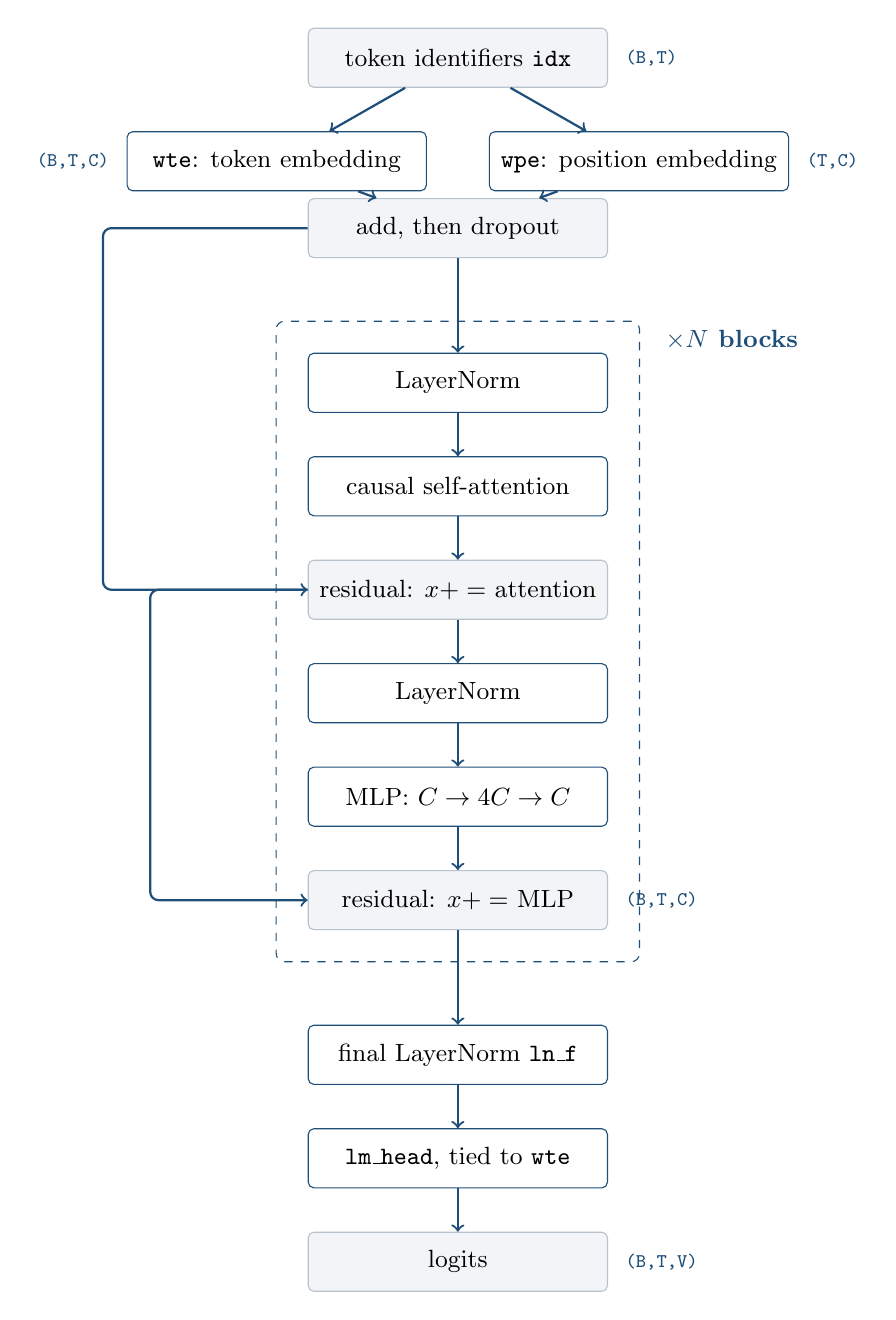
\begin{tikzpicture}[
  node distance=5.5mm,
  box/.style={draw=rule,fill=soft,rounded corners=2pt,minimum width=38mm,
              minimum height=7.5mm,align=center,font=\small},
  op/.style={draw=accent,fill=white,rounded corners=2pt,minimum width=38mm,
             minimum height=7.5mm,align=center,font=\small},
  lbl/.style={font=\scriptsize\ttfamily,text=accent},
  ar/.style={->,draw=accent,thick}
]

\node[box] (idx) {token identifiers \code{idx}};
\node[op,below=of idx,xshift=-23mm] (wte) {\code{wte}: token embedding};
\node[op,below=of idx,xshift=23mm]  (wpe) {\code{wpe}: position embedding};
\node[box,below=14mm of idx] (add) {add, then dropout};

\draw[ar] (idx) -- (wte);
\draw[ar] (idx) -- (wpe);
\draw[ar] (wte) -- (add);
\draw[ar] (wpe) -- (add);
\node[lbl,right=1mm of idx.east] {(B,T)};
\node[lbl,left=1mm of wte.west] {(B,T,C)};
\node[lbl,right=1mm of wpe.east] {(T,C)};

% ---- the block
\node[op,below=12mm of add] (ln1) {LayerNorm};
\node[op,below=of ln1] (attn) {causal self-attention};
\node[box,below=of attn] (res1) {residual: $x \mathbin{+}=$ attention};
\node[op,below=of res1] (ln2) {LayerNorm};
\node[op,below=of ln2] (mlp) {MLP: $C \to 4C \to C$};
\node[box,below=of mlp] (res2) {residual: $x \mathbin{+}=$ MLP};

\draw[ar] (add) -- (ln1);
\draw[ar] (ln1) -- (attn);
\draw[ar] (attn) -- (res1);
\draw[ar] (res1) -- (ln2);
\draw[ar] (ln2) -- (mlp);
\draw[ar] (mlp) -- (res2);

% skip connections
\draw[ar,rounded corners=3pt] (add.west) -- ++(-26mm,0) |- (res1.west);
\draw[ar,rounded corners=3pt] (res1.west) -- ++(-20mm,0) |- (res2.west);

\begin{scope}[on background layer]
  \node[draw=accent,dashed,rounded corners=3pt,inner sep=4mm,
        fit=(ln1)(attn)(res1)(ln2)(mlp)(res2)] (blk) {};
\end{scope}
\node[font=\small\bfseries,text=accent,right=2mm of blk.north east,anchor=north west]
  {$\times N$ blocks};

\node[op,below=12mm of res2] (lnf) {final LayerNorm \code{ln\_f}};
\node[op,below=of lnf] (head) {\code{lm\_head}, tied to \code{wte}};
\node[box,below=of head] (out) {logits};

\draw[ar] (res2) -- (lnf);
\draw[ar] (lnf) -- (head);
\draw[ar] (head) -- (out);
\node[lbl,right=1mm of res2.east] {(B,T,C)};
\node[lbl,right=1mm of out.east] {(B,T,V)};

\end{tikzpicture}
\caption{The data flow from token identifiers to next-token logits. The two residual
connections give an identity path through every block.}
\label{fig:arch}
\end{figure}

The meaning of the output is important. \code{logits[b,t,:]} holds the scores for the token
\textbf{after} position $t$. One forward pass therefore gives a prediction at every position.

The two embeddings answer two different questions. The token embedding answers the question: what
is this character? The position embedding answers the question: where is this character? The model
adds the two vectors. The sum is the start of the residual stream. Every block then reads the
stream and adds a small change to it.

\subsection{Inside causal self-attention}

Table~\ref{tab:shapes} follows one block, from \code{gpt/model.py:52--65}.

\begin{table}[htbp]\centering
\begin{tabular}{@{}lll@{}}
\toprule
\textbf{Step} & \textbf{Operation} & \textbf{Shape} \\
\midrule
Input & \code{x} & \code{(B,T,C)} \\
Project & \code{qkv(x)} & \code{(B,T,3C)} \\
Split & \code{q, k, v} & $3 \times$ \code{(B,T,C)} \\
Separate the heads & \code{view(B,T,H,D).transpose(1,2)} & $3 \times$ \code{(B,H,T,D)} \\
Score & \code{q @ k.T / sqrt(D)} & \code{(B,H,T,T)} \\
Mask & \code{masked\_fill(tril == 0, -inf)} & \code{(B,H,T,T)} \\
Normalize & \code{softmax(dim=-1)} & \code{(B,H,T,T)} \\
Collect the values & \code{weights @ v} & \code{(B,H,T,D)} \\
Join the heads & \code{transpose(1,2).view(B,T,C)} & \code{(B,T,C)} \\
Project & \code{proj(...)} & \code{(B,T,C)} \\
\bottomrule
\end{tabular}
\caption{The tensor shapes through one attention sublayer.}
\label{tab:shapes}
\end{table}

Three points connect my code to the paper.

\paragraph{One matrix for Q, K and V.} I compute the three projections in one \code{nn.Linear} of
width $3C$, and then I split the result. This is equal to three separate matrices. One large
matrix multiplication is faster than three small ones.

\paragraph{Multi-head attention is a reshape and not a loop.} I move the head axis next to the
batch axis with \code{view} and \code{transpose}. All 8 heads then compute in one batched matrix
multiplication. This is the concatenation
$\mathrm{Concat}(\mathrm{head}_1,\dots,\mathrm{head}_h)W^{O}$ from the paper. The reverse reshape
performs the concatenation. My \code{proj} layer is $W^{O}$.

\paragraph{The shape \code{(B,H,T,T)} is the attention map.} Element \code{[b,h,i,j]} is the
weight that head $h$ gives to position $j$ when it computes position $i$. The mask makes the upper
triangle zero. This tensor is also the memory cost of attention. It grows with $T^{2}$, which is
the reason for my context limit of 128.

\subsection{The loss}

I use cross-entropy in \code{gpt/model.py:150}. I flatten the logits to \code{(B*T, V)}. I flatten
the targets to \code{(B*T,)}. I set \code{ignore\_index=-100}.

The loss is the mean negative log-likelihood of the correct next character. It covers all
positions that are not masked. This is the autoregressive factorization in
Equation~\ref{eq:factor}.

\begin{equation}
p(x) = \prod_{t} p(x_t \mid x_{<t})
\label{eq:factor}
\end{equation}

The causal mask makes this correct. Each factor uses only the characters before position $t$.

\subsection{Text generation}

I generate one token at a time in \code{gpt/generate.py} and \code{mol/sample.py}.

\begin{enumerate}[nosep,leftmargin=1.6em]
  \item Run the model on the current sequence.
  \item Take the last position, \code{logits[:, -1, :]}.
  \item Divide the logits by the temperature.
  \item Keep the top $k$ logits, if the caller asks for this.
  \item Apply softmax and sample. If the temperature is 0, take the \code{argmax} instead.
  \item Append the new token.
  \item Stop at \code{<eos>}, or at \code{block\_size}.
\end{enumerate}

I crop the context to the last \code{block\_size} tokens in step 1. A fixed table of 128 position
vectors is therefore sufficient.

\code{mol/sample.py} does the same work for a complete batch. It records the rows that produced
\code{<eos>}. It writes padding into those rows after that point. This makes the generation of
5000 molecules practical.

%======================================================================
\section{Experiments and Findings}

\code{scripts/experiments.py} produces the results in this section. Every table is also in
\code{results/experiments/summary.md}.

\noindent\fcolorbox{rule}{soft}{\parbox{\dimexpr\textwidth-2\fboxsep-2\fboxrule}{%
\textbf{Status.} The values marked \tbd{} are not measured yet. The training run and the
experiment kernel must finish first. I do not write a finding before I see the measurement.}}

\subsection{Training and validation loss}

\begin{table}[htbp]\centering
\begin{tabular}{@{}ll@{}}
\toprule
\textbf{Item} & \textbf{Value} \\
\midrule
Steps & \tbd \\
Final training loss & \tbd \\
Final validation loss & \tbd \\
Parameters & \tbd \\
Run time & \tbd{} minutes on a Kaggle T4 \\
\bottomrule
\end{tabular}
\caption{The main training run.}
\end{table}

\resultfig{../results/smiles_loss.png}{\textwidth}{Left: training and validation loss.
Right: validity, uniqueness and novelty, measured on fresh samples at every evaluation step.}

The left plot shows the two losses. The right plot shows the three generation metrics. I measure
the metrics on fresh samples at every evaluation step.

The second plot is the more useful one. A falling loss shows that the model predicts characters
better. A rising validity shows that the model learned the grammar. The model must close every
bracket and pair every ring digit to produce a valid molecule.

\begin{table}[htbp]\centering
\begin{tabular}{@{}lll@{}}
\toprule
\textbf{Metric} & \textbf{Meaning} & \textbf{Score} \\
\midrule
Validity & the generated strings that RDKit can parse & \tbd \\
Uniqueness & the distinct molecules among the valid ones & \tbd \\
Novelty & the valid molecules that are not in the training set & \tbd \\
\bottomrule
\end{tabular}
\caption{Generation metrics from the final checkpoint.}
\end{table}

\noindent\textbf{Interpretation.} \tbd

\subsection{The effect of temperature}

Temperature divides the logits before the softmax. The effect is a change of shape in the
probability distribution.

\begin{itemize}[nosep,leftmargin=1.4em]
  \item A low temperature makes the distribution sharp. The model almost always takes the most
        probable character.
  \item A high temperature makes the distribution flat. Rare characters become more probable.
  \item Temperature 0 is greedy decoding. The model always takes the most probable character.
\end{itemize}

Greedy decoding has a consequence that I must state. The model gets the same prompt every time. It
therefore produces the same string every time. Uniqueness falls to one molecule.

\resultfig{../results/experiments/temperature.png}{0.72\textwidth}{Validity, uniqueness and
novelty against the sampling temperature.}

\begin{table}[htbp]\centering
\begin{tabular}{@{}llllll@{}}
\toprule
\textbf{Temperature} & \textbf{Validity} & \textbf{Uniqueness} & \textbf{Novelty} &
\textbf{Mean QED} & \textbf{Mean logP} \\
\midrule
0 (greedy) & \tbd & \tbd & \tbd & \tbd & \tbd \\
0.5 & \tbd & \tbd & \tbd & \tbd & \tbd \\
0.7 & \tbd & \tbd & \tbd & \tbd & \tbd \\
0.8 & \tbd & \tbd & \tbd & \tbd & \tbd \\
1.0 & \tbd & \tbd & \tbd & \tbd & \tbd \\
1.2 & \tbd & \tbd & \tbd & \tbd & \tbd \\
1.5 & \tbd & \tbd & \tbd & \tbd & \tbd \\
\bottomrule
\end{tabular}
\caption{The effect of temperature on 2000 unconditional samples per setting.}
\end{table}

\noindent\textbf{Interpretation.} \tbd

\subsection{The effect of prompt length and context}

I made two measurements.

\paragraph{Measurement 1: the loss at each position.} I compute the mean cross-entropy at each
position index over the validation set. The question is simple. Does more context make the next
character easier to predict?

\paragraph{Measurement 2: completion of a real prefix.} I take a molecule from the validation set.
I keep the first $k$ characters. I ask the model to complete the string. I then score the complete
string with RDKit. I use $k$ = 0, 5, 10, 20 and 40. The case $k = 0$ is the unconditional
baseline.

This measurement has two possible outcomes, and both are informative. A long prefix gives the
model more context, so the completion can become more reliable. However, a long prefix also makes
a commitment. A prefix with two open rings must close both rings. The model can fail if it does
not have enough remaining positions.

\resultfig{../results/experiments/context.png}{\textwidth}{Left: mean cross-entropy at each
position index. Right: validity of completions against the prefix length.}

\begin{table}[htbp]\centering
\begin{tabular}{@{}lllll@{}}
\toprule
\textbf{Prefix length} & \textbf{Validity} & \textbf{Uniqueness} & \textbf{Novelty} &
\textbf{Mean length} \\
\midrule
0 & \tbd & \tbd & \tbd & \tbd \\
5 & \tbd & \tbd & \tbd & \tbd \\
10 & \tbd & \tbd & \tbd & \tbd \\
20 & \tbd & \tbd & \tbd & \tbd \\
40 & \tbd & \tbd & \tbd & \tbd \\
\bottomrule
\end{tabular}
\caption{Completion of real validation prefixes at temperature 1.0.}
\end{table}

\noindent\textbf{Interpretation.} \tbd

\subsection{The effect of the architecture}
\label{sec:arch}

I changed one architectural parameter at a time. I held every other parameter constant. I also
held the data subset constant. Any difference in the validation loss therefore comes from the
parameter that I changed.

\begin{table}[htbp]\centering
\begin{tabular}{@{}lll@{}}
\toprule
\textbf{Axis} & \textbf{Values} & \textbf{What it changes} \\
\midrule
\code{n\_layer} & 2, 4, 8 & the depth, which is the number of refinement steps \\
\code{n\_head} & 2, 4, 8 & the number of attention subspaces, at a constant width \\
\code{n\_embd} & 64, 128, 256 & the width of each token representation \\
\bottomrule
\end{tabular}
\caption{The three ablation axes.}
\end{table}

\paragraph{A necessary caveat.} These runs are short. Each run uses 1200 steps on a subset of
200{,}000 molecules, and a limit of 15 minutes. They are a controlled comparison between settings.
They are not converged models. I can therefore make a claim about a relative trend. I cannot make
a claim about the best possible quality.

I first tried these runs on a CPU. After 300 steps the validity was still 0.000. A comparison
between two such models measures noise and not depth. I moved the runs to a GPU for this reason.

\resultfig{../results/experiments/ablation_n_layer.png}{0.72\textwidth}{Depth: validation loss
against \code{n\_layer}.}
\resultfig{../results/experiments/ablation_n_head.png}{0.72\textwidth}{Heads: validation loss
against \code{n\_head}, at constant \code{n\_embd}.}
\resultfig{../results/experiments/ablation_n_embd.png}{0.72\textwidth}{Width: validation loss
against \code{n\_embd}.}

\begin{table}[htbp]\centering
\begin{tabular}{@{}lllll@{}}
\toprule
\textbf{Axis} & \textbf{Value} & \textbf{Parameters} & \textbf{Final validation loss} &
\textbf{Validity} \\
\midrule
\code{n\_layer} & 2 & \tbd & \tbd & \tbd \\
\code{n\_layer} & 4 & \tbd & \tbd & \tbd \\
\code{n\_layer} & 8 & \tbd & \tbd & \tbd \\
\midrule
\code{n\_head} & 2 & \tbd & \tbd & \tbd \\
\code{n\_head} & 4 & \tbd & \tbd & \tbd \\
\code{n\_head} & 8 & \tbd & \tbd & \tbd \\
\midrule
\code{n\_embd} & 64 & \tbd & \tbd & \tbd \\
\code{n\_embd} & 128 & \tbd & \tbd & \tbd \\
\code{n\_embd} & 256 & \tbd & \tbd & \tbd \\
\bottomrule
\end{tabular}
\caption{The effect of three architectural parameters, one at a time.}
\end{table}

A note on the \code{n\_head} sweep. I hold \code{n\_embd} at 256. More heads therefore gives a
smaller head dimension $D = C/H$. With 2 heads, $D$ is 128. With 8 heads, $D$ is 32. This sweep
does not add capacity. It only changes the partition of the same capacity. A non-monotonic result
is therefore possible and interesting. It would show a trade-off between the number of subspaces
and the size of each subspace.

\noindent\textbf{Interpretation.} \tbd

\subsection{Limitations}

\paragraph{Every output is a candidate and not a drug.} A valid SMILES string that resembles the
training distribution proves very little. It does not show that a molecule binds a target. It does
not show that a chemist can synthesize the molecule. It does not show that the molecule is safe.
Those questions need docking simulations and laboratory work. My result is narrower. The model
learned the SMILES grammar and the shape of drug-like chemical space from next-character
prediction alone.

\paragraph{The model does not guarantee validity.} The grammar is learned and not enforced. I
could add a constrained decoder that rejects an illegal character. I did not do this, because
validity is my measurement. An enforced grammar would make the measurement meaningless.

\paragraph{The context is limited to 128 tokens.} Attention costs $T^{2}$ in memory. I dropped
every molecule with more than 100 characters during data preparation.

\paragraph{The dataset is a subset.} I used 600{,}000 molecules and not the complete MOSES set.
RDKit canonicalization and the QED calculation run on one thread. The complete set would use most
of the GPU session for data preparation alone.

\subsection{Implementation challenges}

\paragraph{The attention mask must be applied before the softmax.} A mask after the softmax leaves
rows that do not sum to 1. The output is then not a weighted average, and the loss becomes
difficult to interpret.

\paragraph{A logged number did not match the data in use.} I added a \code{max\_rows} option to
make the ablation runs small. The training script then printed the row count from
\code{meta.json}. That file holds the count before the limit. A capped run therefore reported the
complete dataset size. The numbers in a report must come from the data in use, so I corrected the
script to report the rows that it loads.

\paragraph{The property tokens must not contribute to the loss.} The property tokens are an input
and not a target. I set the target to $-100$ at those two positions. Without this mask the model
would learn to predict the property bin of a molecule that it has not yet written.

\paragraph{A shared value list does not suit three different axes.} My first ablation command
passed one list of values for all three axes. The value 64 is valid for \code{n\_embd}, but the
value 2 is not, because \code{n\_embd} must divide by \code{n\_head}. The script skipped that axis
without an error. I removed the shared list, so each axis now uses its own values.

\subsection{Lessons learned}

\paragraph{A measurement is better than an opinion.} RDKit parses a string, or it does not. This
made the project tractable. I did not need to judge the quality of the output myself.

\paragraph{The correct experiment needs the correct hardware.} I wasted time on a CPU ablation.
The models did not learn enough to be comparable. A short run on a GPU gives a usable comparison.
A long run on a CPU does not.

\paragraph{Shapes are the best documentation.} I wrote the tensor shape in a comment on almost
every line of \code{gpt/model.py}. A shape comment catches an error immediately. The transpose
between \code{(B,T,H,D)} and \code{(B,H,T,D)} is easy to get wrong, and a wrong order mixes the
heads together.

%======================================================================
\section*{References}
\addcontentsline{toc}{section}{References}

\begin{enumerate}[leftmargin=1.8em]
  \item Vaswani, A., et al. (2017). Attention is all you need. \emph{Advances in Neural
        Information Processing Systems}, 30. \url{https://arxiv.org/abs/1706.03762}
  \item Radford, A., et al. (2019). Language models are unsupervised multitask learners.
        \emph{OpenAI}.
  \item Polykovskiy, D., et al. (2020). Molecular Sets (MOSES): a benchmarking platform for
        molecular generation models. \emph{Frontiers in Pharmacology}.
  \item Karpathy, A. (2022). Let's build GPT: from scratch, in code, spelled out.
  \item Alammar, J. (2018). The illustrated Transformer.
        \url{https://jalammar.github.io/illustrated-transformer/}
\end{enumerate}

\end{document}
